\documentclass[letterpaper, 10pt]{article}


\usepackage{amsfonts}
\usepackage{amsmath}
\usepackage{hyperref}
\hypersetup{colorlinks, linkcolor=red, anchorcolor=blue, citecolor=purple}
\usepackage{xcolor}
\usepackage{graphicx}
\usepackage{tikz}
\usetikzlibrary{arrows}
\usetikzlibrary{decorations}
\usepackage{geometry}
\geometry{left=1.cm, right=1.cm, top=1.5cm, bottom=1.5cm}
\usepackage{listings}
\usepackage{algorithm}
\usepackage{algorithmicx}
\usepackage{algpseudocode}


% Dirac Notation: ket and bar
\newcommand{\qbar}{\rangle}
\newcommand{\qket}{\langle}


\begin{document}

\title{Restricted Boltzmann Machine}
\author{}
\date{\today}
\maketitle
\tableofcontents

\vskip 3cm
\begin{figure}[htbp]
\begin{center}
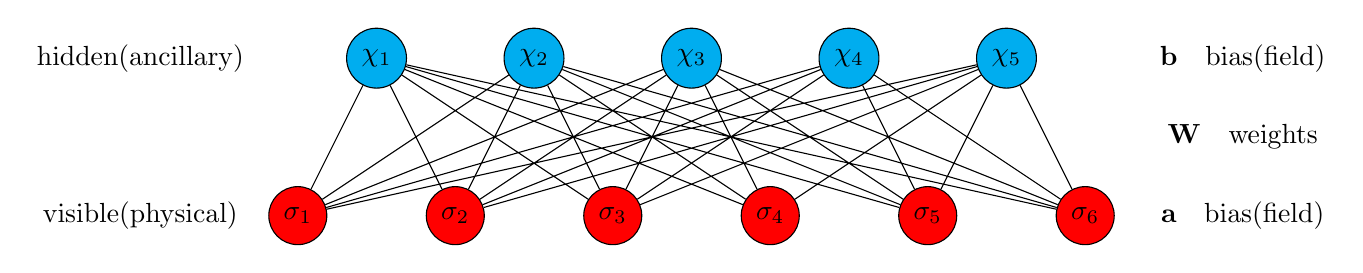
\begin{tikzpicture}
	\draw ( 7,-1) node {\textbf{a}\quad{}\textrm{bias(field)}};
	\draw ( 7, 0) node {\textbf{W}\quad{}\textrm{weights}};
	\draw ( 7, 1) node {\textbf{b}\quad{}\textrm{bias(field)}};
	\draw (-7,-1) node {\textrm{visible(physical)}};
	\draw (-7,1) node {\textrm{hidden(ancillary)}};
	\tikzstyle{every node}=[draw,shape=circle,fill=red];
	\node (s1) at (-5,-1) {$\sigma_1$};
	\node (s2) at (-3,-1) {$\sigma_2$};
	\node (s3) at (-1,-1) {$\sigma_3$};
	\node (s4) at ( 1,-1) {$\sigma_4$};
	\node (s5) at ( 3,-1) {$\sigma_5$};
	\node (s6) at ( 5,-1) {$\sigma_6$};
	\tikzstyle{every node}=[draw,shape=circle,fill=cyan];
	\node (h1) at (-4,1) {$\chi_1$};
	\node (h2) at (-2,1) {$\chi_2$};
	\node (h3) at ( 0,1) {$\chi_3$};
	\node (h4) at ( 2,1) {$\chi_4$};
	\node (h5) at ( 4,1) {$\chi_5$};
	\draw 	(s1)--(h1) (s1)--(h2) (s1)--(h3) (s1)--(h4) (s1)--(h5)
			(s2)--(h1) (s2)--(h2) (s2)--(h3) (s2)--(h4) (s2)--(h5)
			(s3)--(h1) (s3)--(h2) (s3)--(h3) (s3)--(h4) (s3)--(h5)
			(s4)--(h1) (s4)--(h2) (s4)--(h3) (s5)--(h4) (s4)--(h5)
			(s5)--(h1) (s5)--(h2) (s5)--(h3) (s5)--(h4) (s5)--(h5)
			(s6)--(h1) (s6)--(h2) (s6)--(h3) (s6)--(h4) (s6)--(h5);
\end{tikzpicture}
\end{center}
\end{figure}

\newpage
\setcounter{page}{1}


\section{Introduction}
The main task of Machine Learning(ML) is learning from data and making predictions.
There are three main steps in ML:
\begin{itemize}
	\item[1)]
	Collecting the training data set, usually from experiments, our daily life, etc;
	\item[2)]
	Finding a set of functions(also called model, which depends on a set of parameters)
	that is used to represent the law behind the data set;
	\item[3)]
	Defining a loss function to measure the goodness of your function,
	given certain parameter value, and find the best parameter value to minimize the loss function.
\end{itemize}
Considerations on each step can lead to methods with very different models and task-oriented algorithms.


\section[Basic Concepts \& Application]{Basic Concepts \& Application\cite{{melko2016prb},{fischer2012tb}}}

\subsection{Basic Concepts}
Restricted Boltzmann Machine(RBM) is a natural model for studing statistical physics, 
which can be used to learn the probability distribution of a data set.
For a particular configuration $ (\vec{\sigma}, \vec{\chi}) \in \{0,1\}^{N+M} $,
the RBM gives the joint distribution:
\begin{equation}
p(\vec{\sigma},\vec{\chi}) = \frac{1}{Z} \exp{(-E(\vec{\sigma},\vec{\chi}))},
\end{equation}
where the corresponding energy is defined as:
\begin{equation}
E(\vec{\sigma},\vec{\chi}) = 
- \sum_{i=1}^{M} b_i \chi_i - \sum_{j=1}^{N} a_j \sigma_j - \sum_{i,j} W_{ij} \chi_i \sigma_j,
\end{equation}
and $ Z = \sum_{\vec{\sigma},\vec{\chi}} \exp{(-E(\vec{\sigma},\vec{\chi}))} $
is the so-called partition function which is essential to meet the normalization condition.
Then we can get the marginal distribution for the physical configuration \{$ \vec{\sigma} $\}:
\begin{equation}
p(\vec{\sigma}) = \sum_{\vec{\chi}} p(\vec{\sigma},\vec{\chi}) = 
\frac{1}{Z} \exp{( {\color{red}{\sum_{j} a_j \sigma_j}} +
{\color{cyan}{\sum_i \ln{( 1 + \exp{( b_i + \sum_j W_{ij} \sigma_j )} )}}} )} =
\frac{1}{Z} \exp{( - \mathcal{E}(\vec{\sigma}) )}\,, \label{eq:eq1}
\end{equation}
and the {\color{red}{red}} part is just the mean field term,
while the {\color{cyan}{cyan}} part, which is nonlinear, can capture the correlations.
This makes RBM a powerful representation of a very complex probability distribution(indeed,
any distribution with enough hidden units). 
Furthermore, we can calculate conditional distributions using Bayes's theorem as follows:
\begin{eqnarray*}
p(\vec{\sigma}|\vec{\chi})
& = & \frac{\exp{(-E(\vec{\sigma},\vec{\chi}))}/Z}{\sum_{\vec{\sigma}} \exp{(-E(\vec{\sigma},\vec{\chi}))}/Z}
\quad{} \textrm{insert the definition of energy $ E(\vec{\sigma},\vec{\chi}) $} \\
& = & \frac{\prod_{j=1}^{N} \exp{(a_j \sigma_j + \sum_i W_{ij} \chi_i \sigma_j)}}
{\prod_{j=1}^{N} (1 + \exp(a_j + \sum_i W_{ij} \chi_i))} \\
& = & \prod_{j=1}^{N} \frac{\exp{(a_j \sigma_j + \sum_i W_{ij} \chi_i \sigma_j)}}
{1+\exp{(a_j + \sum_i W_{ij} \chi_i)}}\,. \\
\end{eqnarray*}
We can hence reformulate the conditional distributions
in a `decomposed' way(similar for $ p(\vec{\chi}|\vec{\sigma}) $)\footnote{
Attention: the units in the same layer are independent variables when the other layer is fixed.}:
\begin{equation}
p(\vec{\sigma}|\vec{\chi}) = \prod_{j=1}^{N} p(\sigma_j | \vec{\chi})
\quad{} \mathrm{with} \quad{} p(\sigma_j=1 | \vec{\chi}) =
\mathrm{sigmoid}(a_j + \sum_i W_{ij}\chi_i)\,; \label{eq:eq2}
\end{equation}
\begin{equation}
p(\vec{\chi}|\vec{\sigma}) = \prod_{i=1}^{M} p(\chi_i | \vec{\sigma})
\quad{} \mathrm{with} \quad{} p(\chi_i=1 | \vec{\sigma}) =
\mathrm{sigmoid}(b_i + \sum_j W_{ij}\sigma_j)\,.\label{eq:eq3}
\end{equation}
The sigmoid function is defined as: $ \mathrm{sigmoid}(x) = 1/(1+\exp{(-x)}) $\footnote{
In practical programming, $\exp(-x)$ may cause overflow. 
There is another safer version for the sigmoid function as: $ (1+\tanh{(x/2)})/2 $, which is preferred.}. 
An attractive fact about RBM is that: given any configuration $\vec{\sigma}$ as input, 
we can generate a data set(obey the distribution \ref{eq:eq1}) from Markov Chain Monte Carlo(MCMC) 
using the update rules \ref{eq:eq2} and \ref{eq:eq3}.

\subsection{Application}
Our aim is learning the thermodynamics of a classical spin system, 
and all we need to know is the partition function(Ising model for example):
\begin{equation}
Z(\beta) = \sum_{\vec{\sigma}} \exp{( -\beta E(\vec{\sigma}) )}
\quad{} \mathrm{with} \quad{} E(\vec{\sigma}) = -J \sum_{<i,j>} \sigma_i \sigma_j.
\end{equation}
However, it is not practical to calculate it for a general model. 
One can alternatively sample a data set from the corresponding distribution 
$ q(\vec{\sigma}) = \exp{( -\beta E(\vec{\sigma}) )} / Z(\beta) $ 
and average the quantity interested over the data set. 
Here, we generate the data set(training set $ \mathcal{D} $) via conventional Monte Carlo Simulation 
and train the RBM to learn the probability distribution $ q(\vec{\sigma}) $ hidden in the data set, 
finally we sample from the trained RBM and calculate the physical quantities. 
Thus, we need to find parameter value(namely \textbf{W}, \textbf{b}, \textbf{c}) 
which makes the RBM represent the distribution $ q(\vec{\sigma}) $ best. 
Kullback Leibler(KL) divergence is a measure of the distance between two distributions\footnote{
$ -\mathbb{KL}(q||p) = \sum_{\vec{\sigma}} q(\vec{\sigma}) 
\ln{ \frac{p(\vec{\sigma})}{q(\vec{\sigma})} } \leq \ln \sum_{\vec{\sigma}} 
q(\vec{\sigma}) \frac{p(\vec{\sigma})}{q(\vec{\sigma})} = 0 $, 
which uses the Jensen's inequality, and the equality can be obtained via 
$ p(\vec{\sigma})/q(\vec{\sigma}) = \text{const} $, 
together with the normalization condition, 
we finally arrive at: $ \forall \vec{\sigma}, q(\vec{\sigma}) = p(\vec{\sigma}) $.}:
\begin{eqnarray*}
\mathbb{KL}(q||p) 
& = & \sum_{\vec{\sigma}\,\,\textrm{for all}} q(\vec{\sigma}) 
\ln{ \frac{q(\vec{\sigma})}{p(\vec{\sigma})} } \quad{} \textrm{be zero iff } 
q(\vec{\sigma}) = p(\vec{\sigma}) \,\, \textrm{for all }\vec{\sigma} \\
& = & \sum_{\vec{\sigma}\,\,\textrm{for all}} q(\vec{\sigma}) \ln{q(\vec{\sigma})} - \!\!
\sum_{\vec{\sigma}\,\,\textrm{for all}} {\color{cyan}{q(\vec{\sigma})}} \ln{p(\vec{\sigma})} 
\quad{} \textrm{the first term is fixed by the true distribution} \\
& \sim & - \!\!\sum_{\vec{\sigma}\,\,\textrm{for all}} {\color{cyan}{\frac{1}{| \mathcal{D} |} 
\sum_{\vec{\sigma}' \in \mathcal{D}} \delta_{\vec{\sigma},\vec{\sigma}'}}} \ln{p(\vec{\sigma})} 
\quad{} \textrm{note that} \,\, q(\vec{\sigma}) \,\, 
\textrm{can be estimated from the data set $\mathcal{D}$} \\
& = & - \frac{1}{|\mathcal{D}|} \sum_{\vec{\sigma} \in \mathcal{D}} 
\ln p(\vec{\sigma}) \quad{} \textrm{note that the term } 
\sum_{\vec{\sigma} \in \mathcal{D}} \ln p(\vec{\sigma}) = 
\ln \prod_{\vec{\sigma} \in \mathcal{D}} p(\vec{\sigma}) \,\, 
\textrm{is also known as log-likelihood.}
\end{eqnarray*}
The most common strategy to minimize the KL divergence(our loss function) is using Stochastic Gradient Descent(SGD). 
Thus we need to calculate the derivatives of KL divergence with respect to RBM parameters $ \vec{\lambda} $
(attention: we write \{\textbf{W}, \textbf{b}, \textbf{c}\} as $ \vec{\lambda} $):
\begin{equation}
\nabla_{\vec{\lambda}} \, \mathbb{KL}(q||p) = - \frac{1}{|\mathcal{D}|} 
\sum_{\vec{\sigma} \in \mathcal{D}} \nabla_{\vec{\lambda}} \, 
\ln{p_{\vec{\lambda}}(\vec{\sigma})}\,.\label{eq:eq10}
\end{equation}
Here we use $ p_{\vec{\lambda}}(\vec{\sigma}) $ to emphasize the parameter dependence of $ p(\vec{\sigma}) $. 
For each data $ \vec{\sigma}^* $ in data set $ \mathcal{D} $, we have:
\begin{eqnarray*}
\nabla_{\vec{\lambda}} \, \ln{p_{\vec{\lambda}}(\vec{\sigma}^*)}
& = & \nabla_{\vec{\lambda}} \, \ln \frac{1}{Z_{\vec{\lambda}}} 
\sum_{\vec{\chi}} \exp{( - E_{\vec{\lambda}}(\vec{\sigma}^*,\vec{\chi}) )} \\
& = & \nabla_{\vec{\lambda}} \, \ln \sum_{\vec{\chi}} 
\exp{( - E_{\vec{\lambda}}(\vec{\sigma}^*,\vec{\chi}) )} - 
\nabla_{\vec{\lambda}} \ln Z_{\vec{\lambda}} \\
& = & - \frac{\sum_{\vec{\chi}} {\color{red}{\exp{( - E_{\vec{\lambda}}(\vec{\sigma}^*,\vec{\chi}) )}}} 
\nabla_{\vec{\lambda}} \, E_{\vec{\lambda}}(\vec{\sigma}^*,\vec{\chi})}{ {\color{red}{\sum_{\vec{\chi}} 
\exp{( - E_{\vec{\lambda}}(\vec{\sigma}^*,\vec{\chi}) )}}} } + \frac{\sum_{\vec{\sigma},\vec{\chi}} 
{\color{cyan}{\exp{(-E_{\vec{\lambda}}(\vec{\sigma},\vec{\chi}))}}} 
\nabla_{\vec{\lambda}} \, E_{\vec{\lambda}}(\vec{\sigma},\vec{\chi})}{ {\color{cyan}{\sum_{\vec{\sigma},\vec{\chi}} 
\exp{(-E_{\vec{\lambda}}(\vec{\sigma},\vec{\chi}))}}} } \\
& = & - \sum_{\vec{\chi}} {\color{red}{p_{\vec{\lambda}}(\vec{\chi} | \vec{\sigma}^*)}} 
\nabla_{\vec{\lambda}} \, E_{\vec{\lambda}}(\vec{\sigma}^*,\vec{\chi}) + 
\sum_{\vec{\sigma},\vec{\chi}} {\color{cyan}{p_{\vec{\lambda}}(\vec{\sigma},\vec{\chi})}} 
\nabla_{\vec{\lambda}} \, E_{\vec{\lambda}}(\vec{\sigma},\vec{\chi}) \\
& = & - \qket \nabla_{\vec{\lambda}} \, 
E_{\vec{\lambda}}(\vec{\sigma}^*,\vec{\chi})\qbar_{p_{\vec{\lambda}}(\vec{\chi} | 
\vec{\sigma}^*)} + \qket\nabla_{\vec{\lambda}} \, 
E_{\vec{\lambda}}(\vec{\sigma},\vec{\chi})\qbar_{p_{\vec{\lambda}}(\vec{\sigma},\vec{\chi})}\,,
\end{eqnarray*}
the first term is averaged over the conditional distribution for hidden layer 
given a certain $ \vec{\sigma}^* $ which is easy to compute, 
while the second term is averaged over the distribution of the RBM which is difficult to calculate. 
Fortunately, the ML community have already proposed an efficient algorithm 
called contrastive divergence(CD) to estimate the second term. 
Here, we give more detail informations about the derivatives of KL divergence:
\begin{eqnarray}
\nabla_{W_{ij}} \, \ln{p_{\vec{\lambda}}(\vec{\sigma}^*)} 
& = & \qket \chi_i \sigma_j^* \qbar_{{p_{\vec{\lambda}}(\vec{\chi} | \vec{\sigma}^*)}} - 
\qket \chi_i \sigma_j \qbar_{{p_{\vec{\lambda}}(\vec{\chi},\vec{\sigma})}}\label{eq:eq4} \\
\nabla_{a_j} \, \ln{p_{\vec{\lambda}}(\vec{\sigma}^*)} 
& = & \qket \sigma_j^* \qbar_{{p_{\vec{\lambda}}(\vec{\chi} | \vec{\sigma}^*)}} - 
\qket \sigma_j \qbar_{{p_{\vec{\lambda}}(\vec{\chi},\vec{\sigma})}}\label{eq:eq5} \\
\nabla_{b_i} \, \ln{p_{\vec{\lambda}}(\vec{\sigma}^*)} 
& = & \qket \chi_i \qbar_{{p_{\vec{\lambda}}(\vec{\chi} | \vec{\sigma}^*)}} - 
\qket \chi_i \qbar_{{p_{\vec{\lambda}}(\vec{\chi},\vec{\sigma})}}\,.\label{eq:eq6}
\end{eqnarray}
Once we have calculated the derivatives of KL divergence given a certain parameter value, 
we can update the parameters with following rule:
\[ \vec{\lambda}^* = \vec{\lambda} - \eta \nabla_{\vec{\lambda}} \, \mathbb{KL}(\vec{\lambda})\,, \]
where the factor $ \eta $ is the learning rate. 
The SGD will find the best parameter value automatically. 
Once we have trained a RBM, we can use MCMC method to sample from RBM 
which have learned the distribution of training data, 
and compute the physically relevant quantities as follows(denote sampled data set as: $ \mathcal{S} $):
\[ \qket \mathcal{O} \qbar = \frac{1}{|\mathcal{S}|} \sum_{\vec{\sigma} \in \mathcal{S}} \mathcal{O}(\vec{\sigma})\,. \]


\section{Training Algorithm}

\subsection{Gibbs Sampling and Contrastive Divergence}
Now we have all the ingredients needed to train a RBM, 
and the main task is to calculate the values of \ref{eq:eq4}, \ref{eq:eq5} and \ref{eq:eq6}. 
Before we discuss the CD algorithm, it is essential to write these expressions more explicitly. 
For the first one:
\begin{eqnarray}
\nabla_{W_{ij}} \, \ln{p_{\vec{\lambda}}(\vec{\sigma}^*)} 
& = & {\color{cyan}{\sum_{\vec{\chi}} p_{\vec{\lambda}}(\vec{\chi} | \vec{\sigma}^*) \chi_i \sigma_j^*}} - 
\sum_{\vec{\sigma},\vec{\chi}} p_{\vec{\lambda}}(\vec{\sigma},\vec{\chi}) \chi_i \sigma_j 
\quad{} \textrm{using the identity}\,\, \ref{eq:eq3} \nonumber\\
& = & ( \sum_{\chi_i} p_{\vec{\lambda}}(\chi_i | \vec{\sigma}^*) \chi_i \sigma_j^* ) 
\prod_{k \neq i} (\sum_{\chi_k} p_{\vec{\lambda}}(\chi_k | \vec{\sigma}^*)) - 
\sum_{\vec{\sigma},\vec{\chi}} p_{\vec{\lambda}}(\vec{\sigma},\vec{\chi}) \chi_i \sigma_j  \nonumber\\
& = & \sum_{\chi_i} p_{\vec{\lambda}}(\chi_i | \vec{\sigma}^*) \chi_i \sigma_j^* - 
\sum_{\vec{\sigma}} p_{\vec{\lambda}}(\vec{\sigma}) {\color{cyan}{\sum_{\vec{\chi}} 
p_{\vec{\lambda}}(\vec{\chi} | \vec{\sigma}) \chi_i \sigma_j}} \nonumber\\
& = & p_{\vec{\lambda}}(\chi_i=1 | \vec{\sigma}^*) \sigma_j^* - 
\sum_{\vec{\sigma}} p_{\vec{\lambda}}(\vec{\sigma}) p_{\vec{\lambda}}(\chi_i=1 | \vec{\sigma}) \sigma_j \nonumber\\
& = & p_{\vec{\lambda}}(\chi_i=1 | \vec{\sigma}^*) \sigma_j^* - 
\qket p_{\vec{\lambda}}(\chi_i=1 | \vec{\sigma}) \sigma_j \qbar_{p_{\vec{\lambda}}(\vec{\sigma})}\label{eq:eq7}
\end{eqnarray}
Similarly, we have:
\begin{eqnarray}
\nabla_{a_j} \, \ln{p_{\vec{\lambda}}(\vec{\sigma}^*)} 
& = & \sigma_j^* - \qket \sigma_j \qbar_{p_{\vec{\lambda}}(\vec{\sigma})}\label{eq:eq8} \\
\nabla_{b_i} \, \ln{p_{\vec{\lambda}}(\vec{\sigma}^*)} 
& = & p_{\vec{\lambda}}(\chi_i=1 | \vec{\sigma}^*) - 
\qket p_{\vec{\lambda}}(\chi_i=1 | \vec{\sigma})\qbar_{p_{\vec{\lambda}}(\vec{\sigma})}\label{eq:eq9}
\end{eqnarray}
In order to get an average over distribution $ p_{\vec{\lambda}}(\vec{\sigma}) $, 
we can perform a Gibbs sampling\footnote{Start with a specific visible configuration $ \vec{\sigma}^0 $, 
we sample the hidden configuration $ \vec{\chi}^0 $ according to the probability \ref{eq:eq3} given $ \vec{\sigma}^0 $. 
Then we back to sample(reconstruct) the visible configuration $ \vec{\sigma}^1 $ 
according to the probability \ref{eq:eq2} given $ \vec{\chi}^0 $. 
If we do these sampling in order again and again, we will get a long sequence like($ k $-step Gibbs sampling): 
$ \vec{\sigma}^0 \rightarrow \vec{\chi}^0 \rightarrow \vec{\sigma}^1 
\rightarrow \vec{\chi}^1 \rightarrow \cdots \rightarrow \vec{\chi}^{k-1} \rightarrow \vec{\sigma}^k $. 
We refer to the ordered sampling procedure $ \vec{\sigma} \rightarrow \vec{\chi} \rightarrow \vec{\sigma} $ 
as a single step of Gibbs sampling.}. 
However, this is very time-consuming, for you have to do many steps(may be $ \sim 10^3 $ or larger) 
of Gibbs sampling before it reach the equilibrium(convergence). 
CD algorithm uses two tricks to circumvent this difficulty\footnote{The logic is that: 
our ultimate goal is getting a distribution 
$ p_{\vec{\lambda}}(\vec{\sigma}) \sim q(\vec{\sigma}). $ 
If we start Gibbs sampling with a $ \vec{\sigma} $ sampled from $ q(\vec{\sigma}) $, 
it should already arrive at the equilibrium in some sense.}: 
1. start the Gibbs sampling with a $ \vec{\sigma} $ from the training data set, not a random one; 
2. do sampling after only a few steps of Gibbs sampling(in some cases, a single step is good enough!). 
In the spirit of CD algorithm, we can thus replace the average over 
$ p_{\vec{\lambda}}(\vec{\sigma}) $ in \ref{eq:eq7}, \ref{eq:eq8} and \ref{eq:eq9} 
with $ p_{\vec{\lambda}}(\chi_i=1 | \vec{\sigma}^k) \sigma_j^k $, 
$ \sigma_j^k $ and $ p_{\vec{\lambda}}(\chi_i=1 | \vec{\sigma}^k) $, 
where $ \vec{\sigma}^k $ is sampled from $ k $-step Gibbs sampling 
whose starting point is $ \vec{\sigma}^* $\footnote{You may be confused and ask the question that: 
how you can replace the average over a distribution $ p_{\vec{\lambda}}(\vec{\sigma}) $ 
just by one $ \vec{\sigma} $ sampled from it? 
The answer lies in the fact that our derivative of KL divergence includes 
an average(or sum) over the whole data set or a batch in SGD(see expression \ref{eq:eq10}). 
You may convince yourself that this averaging process over training data set or batch 
indeed mimics the averaging process over the distribution $ p_{\vec{\lambda}}(\vec{\sigma}) $.}.

\subsection{Pseudocode For Training Algorithm}
Here I just give a detailed description of the whole training algorithm, see Algorithm \ref{al:rbm}.

\section{Remarks}
The success of RBM is impressive and it is desired to understand the root of its power. 
Recall the energy form defined on the RBM graph, 
\[ E(\vec{\sigma},\vec{\chi}) = - \sum_{i=1}^{M} b_i \chi_i - 
\sum_{j=1}^{N} a_j \sigma_j - \sum_{i,j} W_{ij} \chi_i \sigma_j, \]
it seems that there is no direct interaction between the physical spins. 
However, when we trace out the degrees of ancillary spins, the effective(or free) energy becomes,
\[ \mathcal{E}(\vec{\sigma}) = - \sum_{j} a_j \sigma_j - 
\sum_i \ln{( 1 + \exp{( b_i + \sum_j W_{ij} \sigma_j )} )}, \]
and the correlations between the physical spins just appear. 
Thus the ancillary spins help to correlate the physical spins 
and make the RBM very powerful at representing the Boltzmann distribution. 
On the other hand, however, we can also encode the correlations of physical spins in a direct way. 
In fact, a direct correlation can add nothing to the representation power of the RBM, 
but will destroy the efficiency of the Gibbs sampling which is essential in the training algorithm. 
When the correlation is directly encoded, the `decomposed' form of conditional distribution 
will disappear and makes the Gibb sampling resource consuming(even impossible). 
As a conclusion:
\begin{itemize}
	\item[1)]
	When the information of ancillary spins is unknown(marginal distribution), 
	the physical spins are correlated which makes the RBM very powerful 
	at representing a certain distribution;
	\item[2)]
	When the information of ancillary spins is known(conditional distribution),
	the physcial spins are uncorrelated(independent) which makes the Gibbs sampling very efficient(practical),
\end{itemize}
the correlations between the physical spins must be merely introduced by the ancillary spins! This argument rules out 
the physical and ancillary interactions in the energy from.

\vskip 1cm
\begin{algorithm}[htb]
	\caption{Training of RBM via SGD}\label{al:rbm}
	\begin{algorithmic}[1]
		\Require Data Set $ \mathcal{D} $, RBM's Parameters $ \{\textbf{W}, \textbf{a}, \textbf{b}\} $, 
			Learning Rate $ \eta $, Batch Size $ bs $, Epoch $ ep $, CD Order $ k $, Visible Unit Number: 
			$ N $ and Hidden Unit Number: $M$.
		\Ensure $ \{\textbf{W}^*, \textbf{a}^*, \textbf{b}^*\} = 
			\mathop{\arg\min}_{\vec{\lambda}} \mathbb{KL}(q(\vec{\sigma})||p_{\vec{\lambda}}(\vec{\sigma})) $
		\State Initialize $ \{\textbf{W}, \textbf{a}, \textbf{b}\} $. 
			Each element in $ \textbf{W} $ is sampled from a gaussian distribution: 
			$ W_{ij} \sim \mathcal{N}(0,1)/\sqrt(N+M) $, 
			all the elements in $ \textbf{a}, \textbf{b} $ are set to zero: $ b_i \leftarrow 0, a_j \leftarrow 0 $.
		\State Split $ \mathcal{D} $ into batches $ \mathcal{B} $ randomly, each is of size $ bs $
		\For {$ epoch $ in $ range(1, ep) $}
			\For {each batch $ B $ in $ \mathcal{B} $}
				\State $ \Delta W_{ij}, \Delta a_j, \Delta b_i $ are set to 0, for all $ i, j $
				\For {each data $ \vec{\sigma} $ in batch $ B $}
					\State sample $ \vec{\sigma}^k $ via $ k $-step Gibbs sampling 
						with $ \vec{\sigma} $ as the starting configuration
					\State calculate $ p(\chi_i=1|\vec{\sigma}) $ and $ p(\chi_i=1|\vec{\sigma}^k) $ 
						for all $ i $ via \ref{eq:eq2} and \ref{eq:eq3}
					\State $ \Delta W_{ij} +\!\!= p(\chi_i=1|\vec{\sigma})*\sigma_j - 
						p(\chi_i=1|\vec{\sigma}^k)*\sigma^k_j $
					\State $ \Delta a_j +\!\!= \sigma_j - \sigma_j^k $
					\State $ \Delta b_i +\!\!= p(\chi_i=1|\vec{\sigma}) - p(\chi_i=1|\vec{\sigma}^k) $
				\EndFor
				\State $ W_{ij} \leftarrow W_{ij} + \eta * \Delta W_{ij} / bs $
				\State $ a_j \leftarrow a_j + \eta * \Delta a_j / bs $
				\State $ b_i \leftarrow b_i + \eta * \Delta b_i / bs $
			\EndFor
		\EndFor
	\end{algorithmic}
\end{algorithm}

\section[Road to quantum many-body wave functions]{Road to quantum many-body wave functions\cite{{carleo2017s},{melko2019np}}}
In order to extend the application of RBM to the representation of quantum many-body wave function, we need to consider complex valued parameters:
\[ \phi_{\vec{\lambda}}(\vec{\sigma}) = \frac{1}{\sqrt{Z_{\vec{\lambda}}}} \sum_{\vec{\chi}} \exp{(\sum_{i} b_i \chi_i + \sum_{j} a_j \sigma_j + \sum_{i,j} \chi_i W_{ij} \sigma_j)}. \]
Because we do not have any data for this problem, we need to adopt variational principle:
\begin{itemize}
	\item[1)] Find the ground wave function, we have to minimize the energy function: $E_{\vec{\lambda}} = {\qket \phi_{\vec{\lambda}} | \hat{H} | \phi_{\vec{\lambda}} \qbar}/{\qket \phi_{\vec{\lambda}} | \phi_{\vec{\lambda}} \qbar};$
	\item[2)] Simulate the dynamics of wave function, we have to minimize the distance(parameters becomes time-dependent): $ \mathcal{R}(\dot{\vec{\lambda}}(t)) = \mathrm{dist}(\partial_t | \phi(\dot{\vec{\lambda}}(t)) \qbar, -i \hat{H}| \phi({\vec{\lambda}}(t)) \qbar),$ and it is the time derivative of parameters that we have to learn.
\end{itemize}
The optimization of parameters is performed by Variational Monte Carlo(VMC) and Stochastic Reconfiguration Method(SR), which will be introduced later.

\section[Road to density operator]{Road to density operator(mixed state)\cite{{melko2018prl},{Ciuti2019prl},{Nagy2019prl},{Yoshioka2019prb},{carleo2019prl}}}
In the last section, we know how RBMs can be used to represent a quantum many-body wave function. However, any system in real world must experience decoherence for the coupling with the environment. Thus, it is necessary to know how RBMs can be used to represent a mixed state or density operator. Recently, people proposed three different schemes to achieve this goal.
\subsection[The regular one]{The regular one\cite{{melko2018prl},{Ciuti2019prl}}}
\begin{figure}[htbp]
\begin{center}
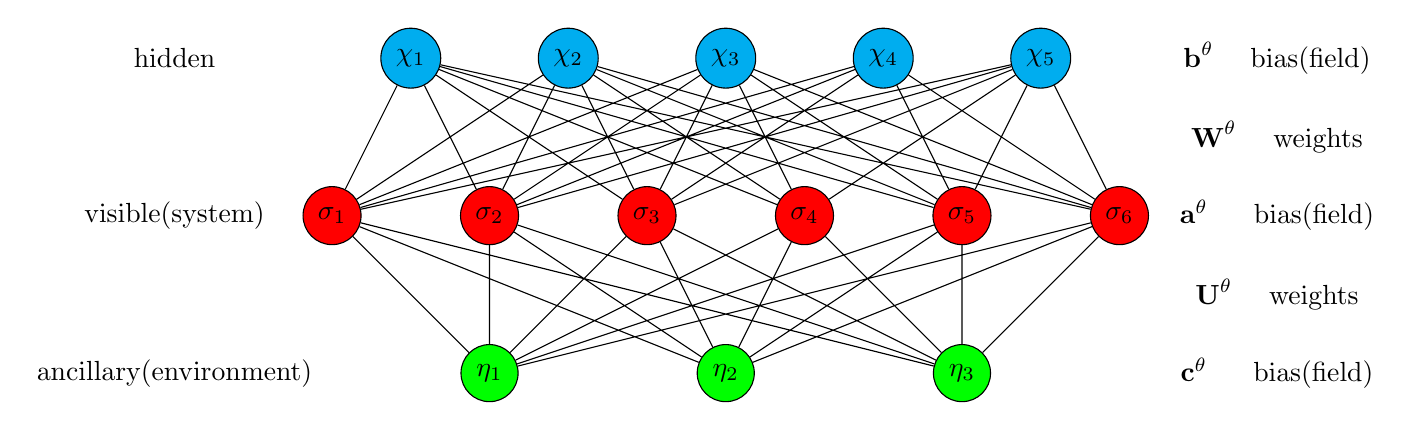
\begin{tikzpicture}
	\draw (7,-1) node {$\textbf{a}^\theta$ \quad{} \textrm{bias(field)}} (7,0) node {$\textbf{W}^\theta$ \quad{}\textrm{weights}} (7,1) node {$\textbf{b}^\theta$ \quad{}\textrm{bias(field)}} (7,-2) node {$\textbf{U}^\theta$\quad{} \textrm{weights}} (7,-3) node {$\textbf{c}^\theta$ \quad{} \textrm{bias(field)}};
	\draw (-7,-1) node {\textrm{visible(system)}} (-7,-3) node {\textrm{ancillary(environment)}} (-7,1) node {\textrm{hidden}};
	\tikzstyle{every node}=[draw,shape=circle,fill=red];
	\node (s1) at (-5,-1) {$\sigma_1$};
	\node (s2) at (-3,-1) {$\sigma_2$};
	\node (s3) at (-1,-1) {$\sigma_3$};
	\node (s4) at (1,-1) {$\sigma_4$};
	\node (s5) at (3,-1) {$\sigma_5$};
	\node (s6) at (5,-1) {$\sigma_6$};
	\tikzstyle{every node}=[draw,shape=circle,fill=cyan];
	\node (h1) at (-4,1) {$\chi_1$};
	\node (h2) at (-2,1) {$\chi_2$};
	\node (h3) at (0,1) {$\chi_3$};
	\node (h4) at (2,1) {$\chi_4$};
	\node (h5) at (4,1) {$\chi_5$};
	\tikzstyle{every node}=[draw,shape=circle,fill=green];
	\node (z1) at (-3,-3) {$\eta_1$};
	\node (z2) at (0,-3) {$\eta_2$};
	\node (z3) at (3,-3) {$\eta_3$};
	\draw 	(s1)--(h1) (s1)--(h2) (s1)--(h3) (s1)--(h4) (s1)--(h5)
			(s2)--(h1) (s2)--(h2) (s2)--(h3) (s2)--(h4) (s2)--(h5)
			(s3)--(h1) (s3)--(h2) (s3)--(h3) (s3)--(h4) (s3)--(h5)
			(s4)--(h1) (s4)--(h2) (s4)--(h3) (s5)--(h4) (s4)--(h5)
			(s5)--(h1) (s5)--(h2) (s5)--(h3) (s5)--(h4) (s5)--(h5)
			(s6)--(h1) (s6)--(h2) (s6)--(h3) (s6)--(h4) (s6)--(h5);
	\draw	(s1)--(z1) (s1)--(z2) (s1)--(z3)
			(s2)--(z1) (s2)--(z2) (s2)--(z3)
			(s3)--(z1) (s3)--(z2) (s3)--(z3)
			(s4)--(z1) (s4)--(z2) (s4)--(z3)
			(s5)--(z1) (s5)--(z2) (s5)--(z3)
			(s6)--(z1) (s6)--(z2) (s6)--(z3);
\end{tikzpicture}
\end{center}
\end{figure}
In order to represent a mixed state, the first step we may take is purifying the system with ancillary freedoms, which is a basic concept in quantum information theory. Thus the whole system(system and environment) can be written as:
\[ | \phi \qbar = \sum_{\vec{\sigma},\vec{\eta}} \phi(\vec{\sigma},\vec{\eta}) | \vec{\sigma} \qbar \otimes | \vec{\eta} \qbar, \]
and the state of system is easily obtained via tracing out the ancillary degrees:
\[ \rho(\vec{\sigma},\vec{\sigma}') = \sum_{\vec{\eta}} \phi(\vec{\sigma},\vec{\eta}) \phi^*(\vec{\sigma}', \vec{\eta}). \]
Here we use two RBMs, which share the same architecture but different parameters(denoted by $\vec{\lambda}$ and $\vec{\gamma}$), to represent the wave function of the whole system:
\[ \phi(\vec{\sigma},\vec{\eta}) = \frac{1}{\sqrt{Z_{\vec{\lambda}}}} \sqrt{p_{\vec{\lambda}}(\vec{\sigma},\vec{\eta})} \exp{(\frac{i}{2} \ln p_{\vec{\gamma}}(\vec{\sigma},\vec{\eta}))}, \]
after tracing out the ancillary degrees, we can get the expression of system's density operator. 

\subsection[The natural one]{The natural one\cite{{Nagy2019prl},{carleo2019prl}}}
\begin{figure}[htbp]
\begin{center}
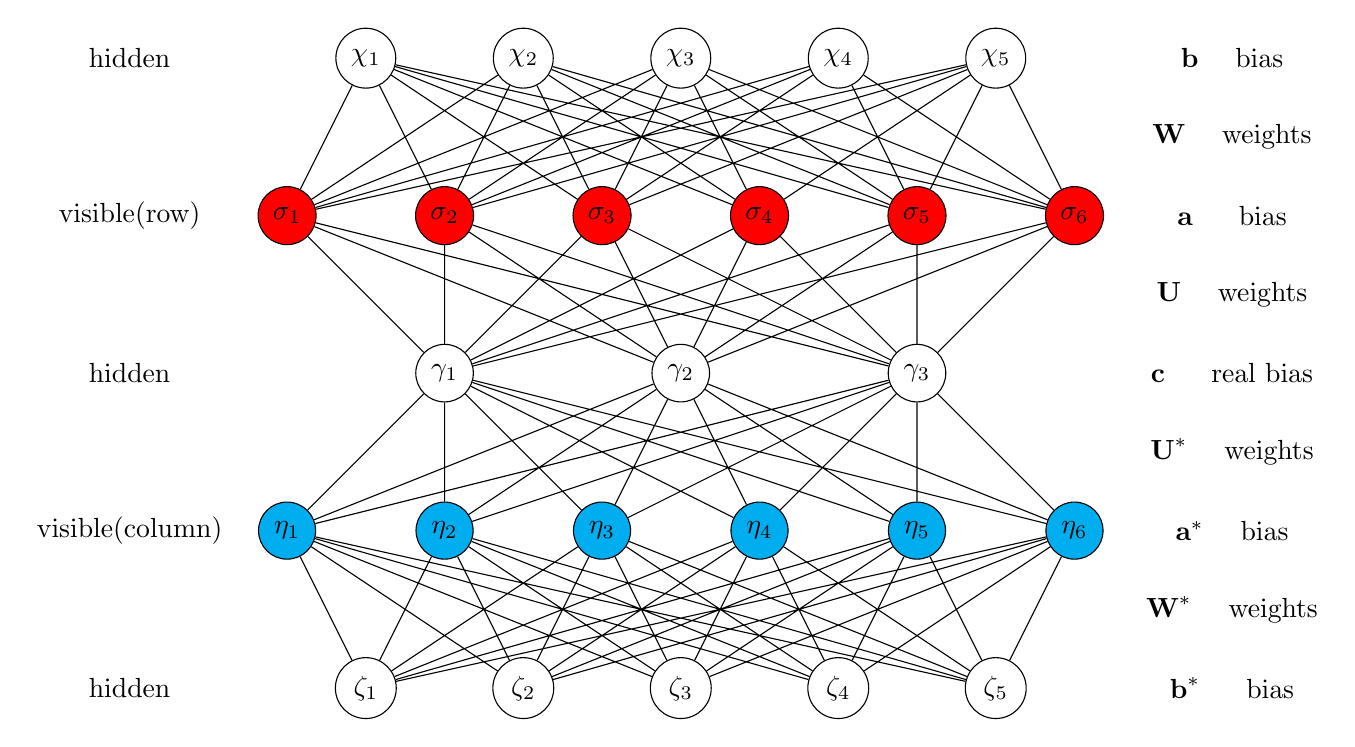
\begin{tikzpicture}
	\draw (7,-1) node {$\textbf{a}$ \quad{} \textrm{bias}} (7,0) node {$\textbf{W}$ \quad{}\textrm{weights}} (7,1) node {$\textbf{b}$ \quad{}\textrm{bias}} (7,-2) node {$\textbf{U}$\quad{} \textrm{weights}} (7,-3) node {$\textbf{c}$ \quad{} \textrm{real bias}} (7,-4) node {$\textbf{U}^*$ \quad{}\textrm{weights}} (7,-5) node {$\textbf{a}^*$ \quad{}\textrm{bias}} (7,-6) node {$\textbf{W}^*$ \quad{}\textrm{weights}} (7,-7) node {$\textbf{b}^*$ \quad{} \textrm{bias}};
	\draw (-7,-1) node {\textrm{visible(row)}} (-7,-3) node {\textrm{hidden}} (-7,1) node {\textrm{hidden}} (-7,-5) node {\textrm{visible(column)}} (-7, -7) node {hidden};
	\tikzstyle{every node}=[draw,shape=circle,fill=red];
	\node (s1) at (-5,-1) {$\sigma_1$};
	\node (s2) at (-3,-1) {$\sigma_2$};
	\node (s3) at (-1,-1) {$\sigma_3$};
	\node (s4) at (1,-1) {$\sigma_4$};
	\node (s5) at (3,-1) {$\sigma_5$};
	\node (s6) at (5,-1) {$\sigma_6$};
	\tikzstyle{every node}=[draw,shape=circle];
	\node (h1) at (-4,1) {$\chi_1$};
	\node (h2) at (-2,1) {$\chi_2$};
	\node (h3) at (0,1) {$\chi_3$};
	\node (h4) at (2,1) {$\chi_4$};
	\node (h5) at (4,1) {$\chi_5$};
	\tikzstyle{every node}=[draw,shape=circle];
	\node (z1) at (-3,-3) {$\gamma_1$};
	\node (z2) at (0,-3) {$\gamma_2$};
	\node (z3) at (3,-3) {$\gamma_3$};
	\tikzstyle{every node}=[draw,shape=circle,fill=cyan];
	\node (c1) at (-5, -5) {$\eta_1$};
	\node (c2) at (-3, -5) {$\eta_2$};
	\node (c3) at (-1, -5) {$\eta_3$};
	\node (c4) at (1, -5) {$\eta_4$};
	\node (c5) at (3, -5) {$\eta_5$};
	\node (c6) at (5, -5) {$\eta_6$};
	\tikzstyle{every node}=[draw,shape=circle];
	\node (e1) at (-4 , -7) {$\zeta_1$};
	\node (e2) at (-2, -7) {$\zeta_2$};
	\node (e3) at (0, -7) {$\zeta_3$};
	\node (e4) at (2, -7) {$\zeta_4$};
	\node (e5) at (4, -7) {$\zeta_5$};
	\draw 	(s1)--(h1) (s1)--(h2) (s1)--(h3) (s1)--(h4) (s1)--(h5)
			(s2)--(h1) (s2)--(h2) (s2)--(h3) (s2)--(h4) (s2)--(h5)
			(s3)--(h1) (s3)--(h2) (s3)--(h3) (s3)--(h4) (s3)--(h5)
			(s4)--(h1) (s4)--(h2) (s4)--(h3) (s5)--(h4) (s4)--(h5)
			(s5)--(h1) (s5)--(h2) (s5)--(h3) (s5)--(h4) (s5)--(h5)
			(s6)--(h1) (s6)--(h2) (s6)--(h3) (s6)--(h4) (s6)--(h5);
	\draw	(s1)--(z1) (s1)--(z2) (s1)--(z3)
			(s2)--(z1) (s2)--(z2) (s2)--(z3)
			(s3)--(z1) (s3)--(z2) (s3)--(z3)
			(s4)--(z1) (s4)--(z2) (s4)--(z3)
			(s5)--(z1) (s5)--(z2) (s5)--(z3)
			(s6)--(z1) (s6)--(z2) (s6)--(z3);
	\draw	(z1)--(c1) (z1)--(c2) (z1)--(c3) (z1)--(c4) (z1)--(c5) (z1)--(c6)
			(z2)--(c1) (z2)--(c2) (z2)--(c3) (z2)--(c4) (z2)--(c5) (z2)--(c6)
			(z3)--(c1) (z3)--(c2) (z3)--(c3) (z3)--(c4) (z3)--(c5) (z3)--(c6);
	\draw	(e1)--(c1) (e1)--(c2) (e1)--(c3) (e1)--(c4) (e1)--(c5) (e1)--(c6)
			(e2)--(c1) (e2)--(c2) (e2)--(c3) (e2)--(c4) (e2)--(c5) (e2)--(c6)
			(e3)--(c1) (e3)--(c2) (e3)--(c3) (e3)--(c4) (e3)--(c5) (e3)--(c6)
			(e4)--(c1) (e4)--(c2) (e4)--(c3) (e4)--(c4) (e4)--(c5) (e4)--(c6)
			(e5)--(c1) (e5)--(c2) (e5)--(c3) (e5)--(c4) (e5)--(c5) (e5)--(c6);
\end{tikzpicture}
\end{center}
\end{figure}
A natural way to represent a density operator is using one layer to encode the correlations within row degrees or column degrees, and another layer for the mixture of row and column degrees as\footnote{In order to satisfy the conditions of density operator, there must be some constraints on the RBM, like the conjugation of parameters, the symmetry of the structure, etc.}:
\begin{eqnarray*}
\rho(\vec{\sigma},\vec{\eta}) & = & \sum_{\vec{\chi},\vec{\gamma},\vec{\zeta}} \exp(\vec{c} \cdot \vec{\gamma}) \times \exp(\vec{a} \cdot \vec{\sigma} + \vec{b} \cdot \vec{\chi} + \vec{\chi} \cdot W \vec{\sigma} + \vec{\gamma} \cdot U \vec{\sigma}) \times \exp(\vec{a}^* \cdot \vec{\eta} + \vec{b}^* \cdot \vec{\zeta} + \vec{\zeta} \cdot W^* \vec{\eta} + \vec{\gamma} \cdot U^* \vec{\eta})
\end{eqnarray*}
Obviously, this method is more natural than the first one and we don't need the domain knowledge about state purification from quantum information. However, we have to do this at the cost of using complex parameters.

\subsection[The `lazy' one]{The `lazy' one\cite{{Yoshioka2019prb}}}
Further more, there is also a `lazy' way to represent the density matrix of the system. If we trust in the power of RBM, we can use the original structure\footnote{With complex and conjugate parameters of course.}! We just equally split the visible layers into two parts, one for row and the other for column,
\[ \rho(\vec{\sigma},\vec{\eta}) = \frac{1}{Z} \sum_{\vec{\chi}} \exp(\vec{a} \cdot \vec{\sigma} + \vec{a}^* \cdot \vec{\eta} + \vec{b} \cdot \vec{\chi} + \vec{\chi} \cdot W \vec{\sigma} + \vec{\chi} \cdot W^* \vec{\eta}).  \]
 Although we have applied some constraints on the RBM, it is not generally to be a legal density matrix\footnote{Positive-semidefinite and hermitian. Queation: why not use real $\vec{b}$ instead of complex $\vec{b}$ ?}. We believe that the optimization procedure will help us find the stationary state which is legal.

\subsection{Map the optimization problem to a familiar one}
The open quantum system is usually described by the so called Lindblad master equation for the reduced density matrix of the system:
\[ \dot{\rho} = \mathcal{L} \rho, \]
and the stationary state is determined by the condition $ \mathcal{L} \rho = 0.$ As we do in HEOM, we can reshape the density matrix to be a vector and the super-operator $\mathcal{L}$ to be a matrix, then the target state is just the eigenstate of the super-operator with eigenvalue $0$. Furthermore, the eigenstates other than the stationary one will have a negative value on their real part eigenvalues, which agrees with the physical picture that they will eventually decay to be zero in the dynamical evolution. Thus if we consider the super-operator $\mathcal{L}^\dag \mathcal{L}$ which is positive-semidefinite and hermitian, we will find that the stationary state is just the ground state of the ``hamiltonian" $\mathcal{L}^\dag \mathcal{L}$ with exact zero eigenvalue!

\section{Variational Monte Carlo method}

\subsection{Basic ideals of VMC}
Assume we have a trial wave-function $|\phi\qbar$ with parameters $\vec{\alpha}$, we can expand it in the computational basis as:
\[ | \phi \qbar = \sum_{\vec{\sigma}} |\vec{\sigma}\qbar \qket \vec{\sigma}| \phi \qbar = \sum_{\vec{\sigma}} \phi(\vec{\sigma}) | \vec{\sigma} \qbar. \]
Thus we can compute any quantum observable $\hat{O}$ via:
\begin{equation}
\qket \hat{O} \qbar = \frac{\qket \phi | \hat{O} | \phi \qbar}{\qket \phi | \phi \qbar} = \frac{\sum_{\vec{\sigma}} \qket \phi | \vec{\sigma} \qbar \qket \vec{\sigma} | \hat{O} | \phi \qbar}{\sum_{\vec{\sigma}} \qket \phi | \vec{\sigma} \qbar \qket \vec{\sigma} | \phi \qbar} = \frac{\sum_{\vec{\sigma}} | \phi(\vec{\sigma}) |^2 O_\text{loc}(\vec{\sigma})}{\sum_{\vec{\sigma}} | \phi(\vec{\sigma}) |^2},
\label{eq:eq4}
\end{equation}
the local observable $O_\text{loc}(\vec{\sigma})$ is defined by:
\[ O_\text{loc}(\vec{\sigma}) = \frac{\qket \vec{\sigma} | \hat{O} | \phi \qbar}{\qket \vec{\sigma} | \phi \qbar}. \]
However, it's impractical to sum over all the exponential numbered configurations. An alternative approach might be to sum over a set of configurations $\mathcal{S}$ sampled from the distribution $p(\vec{\sigma}) \propto | \phi(\vec{\sigma}) |^2$, and the formula \ref{eq:eq4} can be approximated as:
\begin{equation}
\qket \hat{O} \qbar \approx \frac{1}{|\mathcal{S}|} \sum_{\vec{\sigma} \in \mathcal{S}} O_\text{loc}(\vec{\sigma}).
\label{eq:eq5}
\end{equation}
In undergraduate quantum mechanical class, we have learned the variational principle as ($| n \qbar$ are the eigenstates of system's hamiltonian, and ordered by the eigenvalues as $E_0 \leq E_1 \leq \cdots \leq E_N $):
\[ E_\phi = \frac{\qket \phi | \hat{H} | \phi \qbar}{\qket \phi | \phi \qbar} = \frac{\sum_{n=0}^{N} E_n \qket \phi | n \qbar \qket n | \phi \qbar}{\qket \phi | \phi \qbar} \geq \frac{E_0 \sum_{n=0}^{N}  \qket \phi | n \qbar \qket n | \phi \qbar}{\qket \phi | \phi \qbar} = E_0,\]
which states that the energy of a wave-function is bounded from below by the exact ground energy. The best choice of the parameters $\vec{\alpha}$ - the one makes the trial wave-function as close as possible to the ground state - is the one minimize the value of $E_\phi$. Obviously, a good variational wave-function will be the key to the accuracy of our result. A bad variational wave-function can never be a good approximation of the ground state! In practical applications, people usually impose some constraints or forms to the variational function known from other analytic or symmetry considerations, like Hartree-Fock technique or Density functional theory. However, RBM is a very powerful representation of the wave-function, we have no need to do other complicated analysis to make the guess function have the similar form as the target one. Anyway, we have two main steps in our VMC algorithm:
\begin{itemize}
	\item[1)] Find the best parameters $\vec{\alpha}$ which minimize the value $E_\phi$;
	\item[2)] Calculate the quantities interested via formula \ref{eq:eq4} and \ref{eq:eq5}.
\end{itemize}
Now, there are still two questions we have to answer:
\begin{itemize}
	\item[1)] How to sample the set of configuration $\mathcal{S}$ from the distribution $p(\vec{\sigma}) \propto | \phi(\vec{\sigma}) |^2$;
	\item[2)] How to find the best parameters $\vec{\alpha}$ for the ground state problem.
\end{itemize}
We will solve the first one in this section and leave the second one till the next section.

\subsection{Importance sampling of spin configurations}
The importance sampling of configurations is just similar as the Monte Carlo simulation of classical spin systems, and the only modification is the acceptance should be replaced by:
\[ p(\vec{\sigma} \rightarrow \vec{\sigma}') = \min ( 1, \frac{|\phi(\vec{\sigma}')|^2}{|\phi(\vec{\sigma})|^2} ). \]
\section{Stochastic reconfiguration method}
Our trial wave-function $|\phi\qbar$ is dependent on a set of parameters $\vec{\alpha} = \{ \alpha_1, \alpha_2, \cdots, \alpha_p \}$, and we want to get the best $\vec{\alpha}$ to make $|\phi\qbar$ represent the ground state as close as possible. RS method tells us how to move in the parameter space to minimize the energy by an iterative way. For the trial wave-function $|\phi\qbar$ not orthogonal to the ground state, it is always possible to obtain a new state closer to the ground state by applying the operator $(\Lambda - \hat{H})$ to $|\phi\qbar$ with a sufficient large $\Lambda$ at least bigger than the largest eigenvalue of hamiltonian. The basic ideal of SR is to change the parameters of $|\phi\qbar$ in order to be close as possible as $(\Lambda - \hat{H})|\phi\qbar$. We set the new state to be the following form\footnote{In order to be close as possible as $(\Lambda - \hat{H})|\phi\qbar$, $\delta \alpha_k$ will not be a infinitesimal quantity, and a factor $\delta \alpha_0 \sim \Lambda$ is necessary before $|\phi\qbar$. However, they can point the desired trajectory in the parameter space and the updating formula needs a factor less than $\Lambda^{-1}$ to ensure the convergence.}:
\[ |\phi' \qbar = \delta\alpha_0 |\phi\qbar + \sum_{k=1}^p \delta\alpha_k \frac{\partial |\phi\qbar}{\partial \alpha_k}. \]
This formula can be written in a more compact way as:
\begin{eqnarray*}
|\phi'\qbar & = & \delta\alpha_0 |\phi\qbar + \sum_{k=1}^p \delta\alpha_k \frac{\partial}{\partial \alpha_k} \sum_{\vec{\sigma}} |\vec{\sigma}\qbar\qket\vec{\sigma}|\phi\qbar\\
                 & = & \delta\alpha_0 |\phi\qbar + \sum_{k=1}^p \delta\alpha_k \sum_{\vec{\sigma}} \frac{\partial \ln \phi(\vec{\sigma})}{\partial \alpha_k} |\vec{\sigma}\qbar\qket\vec{\sigma}|\phi\qbar\\
                 & = & \sum_{k=0}^p \delta\alpha_k \hat{\Delta}_{\phi k} |\phi\qbar.\\
\hat{\Delta}_{\phi k} & := & \begin{cases} \mathbb{I} & \text{for } k = 0\\ \sum_{\vec{\sigma}} \frac{\partial \ln \phi(\vec{\sigma})}{\partial \alpha_k} |\vec{\sigma}\qbar\qket\vec{\sigma}| & \text{for } k \neq 0 \end{cases}
\end{eqnarray*}
Thus, we can get the following equation:
\[ {\color{red}{\qket\phi| \hat{\Delta}_{\phi k}}} \sum_{k'=0}^p \delta\alpha_{k'} \sum_{\vec{\sigma}} \hat{\Delta}_{\phi k'} |\phi\qbar = {\color{red}{\qket\phi| \hat{\Delta}_{\phi k}}} (\Lambda - \hat{H})|\phi\qbar. \]
Set the $k$ to be zero, we have:
\[ \delta\alpha_0 = \Lambda - \qket \hat{H} \qbar - \sum_{k'=1}^p \delta \alpha_{k'} \qket \hat{\Delta}_{\phi k'} \qbar \sim \Lambda. \]
Now we can substitute the value of $\delta\alpha_0$ for the case $k \neq 0$:
\[
(\Lambda - \qket \hat{H} \qbar - \sum_{k'=1}^p \delta\alpha_{k'} \qket \hat{\Delta}_{\phi k'} \qbar) \qket \hat{\Delta}_{\phi k} \qbar + \sum_{k'=1}^p \delta\alpha_{k'} \qket \hat{\Delta}_{\phi k} \hat{\Delta}_{\phi k'} \qbar = \Lambda \qket \hat{\Delta}_{\phi k} \qbar - \qket \hat{\Delta}_{\phi k} \hat{H} \qbar
\]
\[ \Downarrow \]
\[
\sum_{k'=1}^p \delta\alpha_{k'} (\qket \hat{\Delta}_{\phi k} \hat{\Delta}_{\phi k'} \qbar - \qket \hat{\Delta}_{\phi k'} \qbar \qket \hat{\Delta}_{\phi k} \qbar) = \qket \hat{H} \qbar \qket \hat{\Delta}_{\phi k} \qbar - \qket \hat{\Delta}_{\phi k} \hat{H} \qbar.
\]
By defining the tensor $\stackrel{\leftrightarrow}{S}$ and vector $\vec{f}$ as:
\begin{eqnarray*}
\stackrel{\leftrightarrow}{S}_{k k'} & = & \qket \hat{\Delta}_{\phi k} \hat{\Delta}_{\phi k'} \qbar - \qket \hat{\Delta}_{\phi k'} \qbar \qket \hat{\Delta}_{\phi k} \qbar;\\
\vec{f}_k & = & \qket \hat{H} \qbar \qket \hat{\Delta}_{\phi k} \qbar - \qket \hat{\Delta}_{\phi k} \hat{H} \qbar,
\end{eqnarray*}
we finally come to the core formula of SR method\footnote{The inverse of tensor $\stackrel{\leftrightarrow}{S}$ may be ill defined, so we often add a small identity term to ensure the legality of the inverse operation as: $\stackrel{\leftrightarrow}{S} + \epsilon \mathbb{I}$, and good results can be obtained with $\epsilon \leq 10^{-4}$. Further the inverse of $\stackrel{\leftrightarrow}{S}$ is very hard for large number of parameters, which is a constraint.}:
\[ \stackrel{\leftrightarrow}{S} \delta \vec{\alpha} = \vec{f}. \]
In order to calculate $\delta \vec{\alpha}$, we need to know the expectation values in $\stackrel{\leftrightarrow}{S}$ and $\vec{f}$. Fortunately, they can all be approximated using the formula \ref{eq:eq5}. The corresponding local observables are:
\begin{eqnarray*}
\frac{\qket \vec{\sigma} | \hat{\Delta}_{\phi k} |\phi\qbar}{\qket\vec{\sigma}|\phi\qbar} & = & \frac{\qket \vec{\sigma} | \sum_{\vec{\sigma}'} \frac{\partial \ln \phi(\vec{\sigma}')}{\partial \alpha_k} |\vec{\sigma}'\qbar\qket\vec{\sigma}'|\phi\qbar}{\qket \vec{\sigma} | \phi \qbar} \,\,\,\,\,=\,\,\,\,\, \frac{\partial \ln \phi(\vec{\sigma})}{\partial \alpha_k};\\
\frac{\qket \vec{\sigma} | \hat{\Delta}_{\phi k} \hat{\Delta}_{\phi k'} |\phi\qbar}{\qket\vec{\sigma}|\phi\qbar} & = & \frac{\qket \vec{\sigma} | \sum_{\vec{\sigma}'} \frac{\partial \ln \phi(\vec{\sigma}')}{\partial \alpha_k} |\vec{\sigma}'\qbar\qket\vec{\sigma}'| \sum_{\vec{\sigma}''} \frac{\partial \ln \phi(\vec{\sigma}'')}{\partial \alpha_k'} |\vec{\sigma}''\qbar\qket\vec{\sigma}''| \phi\qbar}{\qket \vec{\sigma} | \phi \qbar} \,\,\,\,\,=\,\,\,\,\, \frac{\partial \ln \phi(\vec{\sigma})}{\partial \alpha_k} \frac{\partial \ln \phi(\vec{\sigma})}{\partial \alpha_k'}\\
\frac{\qket \vec{\sigma} | \hat{\Delta}_{\phi k} \hat{H} |\phi\qbar}{\qket\vec{\sigma}|\phi\qbar} & = & \frac{\qket \vec{\sigma} | \sum_{\vec{\sigma}'} \frac{\partial \ln \phi(\vec{\sigma}')}{\partial \alpha_k} |\vec{\sigma}'\qbar\qket\vec{\sigma}'| \hat{H}| \phi\qbar}{\qket \vec{\sigma} | \phi \qbar} \,\,\,\,\,=\,\,\,\,\, \frac{\partial \ln \phi(\vec{\sigma})}{\partial \alpha_k} E_{\text{loc}}(\vec{\sigma})
\end{eqnarray*}
Finally, our updating formula for the parameters is:
\[ \vec{\alpha}' = \vec{\alpha} + \Delta t \delta \vec{\alpha}, \]
where $\Delta t \leq 1/\Lambda$ is a sufficient small factor to ensure the convergence.

\section[Conclusion]{Conclusion}
So far, we have presented the basic ideal of using the model borrowed from machine learning to solve the quantum many-body physics. Besides the use of restricted Boltzmann machine, there are also many recent works which use other neural networks, like the convolutional neural network\cite{Titus2019prb} and recurrent neural network\cite{Mohamed2020prr,Roth2020arx}, to calculate the ground states of local Hamiltonians. It would be interesting to explore more connections between the many-body physics and machine learning in the future! 

\vskip 2cm
\centering
\begin{thebibliography}{99}
\bibitem{melko2016prb} Learning Thermodynamics with Boltzmann Machines, G. Torlai, R.G. Melko, \href{https://arxiv.org/abs/1606.02718}{arXiv:1606.02718v1}
\bibitem{fischer2012tb} An Introduction to Restricted Boltzmann Machines, A. Fischer, C. Igel
\bibitem{carleo2017s} Solving the Quantum Many-Body Problem with Artificial Neural Networks, G. Carleo, etc, Science.355.602(2017)
\bibitem{melko2019np} Restricted Boltzmann machines in quantum physics, R. G. Melko, etc, Nature Physics.15.887–892(2019)
\bibitem{melko2018prl} Latent Space Purification via Neural Density Operators, G. Torlai, R. G. Melko, PhysRevLett.120.240503(2018)
\bibitem{Ciuti2019prl} Variational neural network ansatz for steady states in open quantum systems, F. Vicentini, A. Biella, etc, PhysRevLett.122.250503(2019)
\bibitem{Nagy2019prl} Variational Quantum Monte Carlo Method with a Neural-Network Ansatz for Open Quantum Systems, A. Nagy, V. Savona, PhysRevLett.122.250501(2019)
\bibitem{Yoshioka2019prb} Constructing neural stationary states for open quantum many-body systems, N. Yoshioka, R. Hamazaki, PhysRevB.99.214306(2019)
\bibitem{carleo2019prl} Neural-Network Approach to Dissipative Quantum Many-Body Dynamics, M. J. Hartmann, G. Carleo, PhysRevLett.122.250502(2019)
\bibitem{Titus2019prb} Two-dimensional frustrated $J_1$-$J_2$ model studied with neural network quantum states, Kenny Choo, Titus Neupert, and Giuseppe Carleo, Phys.Rev.B100,125124(2019)
\bibitem{Mohamed2020prr} Recurrent neural network wave functions, Mohamed Hibat-Allah, Martin Ganahl, Lauren E. Hayward, etc, Phys.Rev.Research2,023358(2020)
\bibitem{Roth2020arx} Iterative Retraining of Quantum Spin Models Using Recurrent Neural Networks, Christopher Roth, \href{https://arxiv.org/abs/2003.06228}{arXiv:2003.06228}
\end{thebibliography}

\end{document}
